% ================================================================================================================================== %
% -------------------------------------------------------------- UART -------------------------------------------------------------- %
% ================================================================================================================================== %

\section{Analiza interfejsu komunikacyjnego}

Interfejs UART jest dzisiaj dostępny w~niemal wszystkich obecnych na rynku mikrokontrolerach oraz w~wielu układach typu SoC. Jego popularność wynika zarówno z~(jak sama nazwa wskazuje) uniwersalnego charakteru jak i~prostoty implementacji. UART to cyfrowe urządzenie peryferyjne umożliwiające szeregową komunikację asynchroniczną. W~większości implementacji parametry komunikacji takie jak szybkość, czy format danych mogą być konfigurowane poprzez zmianę wartości odpowiednich rejestrów sterujących. Nierzadko możliwe jest też ustawienie trybu komunikacji spośród \textit{simplex}, \textit{duplex} lub ~\textit{half-duplex}. Interfejsy tego typu, szczególnie w~zastosowaniach przemysłowych, są często sprzęgane z~konwerterami poziomów logicznych odpowiednich dla standardów RS-232 lub RS-485.

\begin{figure}[ht]
    \centering
    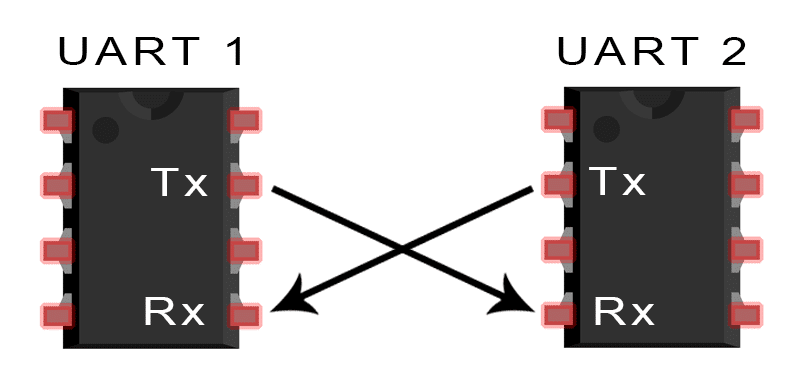
\includegraphics[scale=0.5]{img/theoretical-analysis/uart.png}
    \captionsetup{format=plain,justification=centering}
    \caption{Typowa struktura komunikacji dwóch węzłów z~wykorzystaniem układu UART, źródło: \cite{uart}}
    \label{uart}
\end{figure}

Komunikacja asynchroniczna wymaga aby wszystkie węzły nadawały i~odbierały dane o~z~góry ustalonym formacie i~długości znaku (wynikającym z~szybkości transmisji). Ponadto należy wziąć pod uwagę, że zegary obecne w~poszczególnych urządzeniach mogą się z~czasem rozsynchronizowywać, a~co za tym idzie konieczny jest mechanizm ponownej synchronizacji. W~przypadku komunikacji z~wykorzystaniem modułu UART mechanizm ten wynika z~formatu przesyłanych danych. Typowa ramka składa się z~trzech elementów: \textbf{bitu startu}, \textbf{bitów danych} oraz \textbf{bitów stopu}. Bit startu oznacza początek nowej ramki i~jest sygnalizowany zmianą stanu linii ze spoczynkowego na aktywny. Po nim następuje pewna liczba bitów danych - zazwyczaj $7$ lub $8$  - a~na końcu jeden lub dwa bity stopu. Bit startu odpowiada za synchronizację zegarów wykorzystywanych do próbkowania stanu linii, natomiast bity stopu definiują minimalną przerwę między kolejnymi ramkami. Fakt że każdy bit startu to ponowna okazja do zsynchronizowania zegarów sprawia, że nie muszą one pracować z~dokładnie tymi samymi szybkościami. Niewielkie różnice nie powodują błędów w~odbiorze danych.

\begin{figure}[ht]
    \centering
    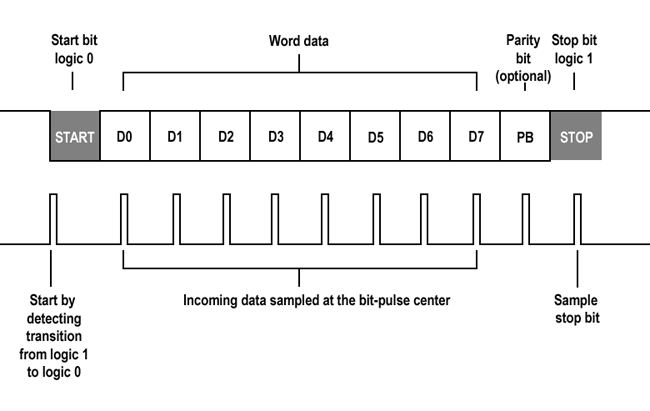
\includegraphics[scale=0.5]{img/theoretical-analysis/uart_frame.png}
    \captionsetup{format=plain,justification=centering}
    \caption{Struktura ramki UART, źródło: \cite{uart_frame}}
    \label{uart-frame}
\end{figure}

Format ramki może zostać rozszerzony o~element kontrolny w~postaci \textbf{bitu parzystości}. Jeśli występuje, przyjmuje on wartość zależną od ilości bitów w~stanie wysokim w~przesyłanych danych i~znajduje się przed bitami stopu. Możliwy jest bit parzystości (ang. \textit{even}) - ustawiony, gdy ilość ta jest parzysta - lub nieparzystości (ang. \textit{odd}) - ustawiany w~przypadku przeciwnym. Dodatkowy element pozwala wykrywać ewentualne błędy transmisji. Format ramki często oznacza się w~postaci trzyznakowego identyfikatora postaci $DPS$, gdzie $D$ oznacza ilość bitów danych, $P$ - typ bitu kontrolnego ($E$ - bit parzystości, $O$ - bit nieparzystości, $N$ - brak bitu kontrolnego) a~$S$ ilość bitów stopu. Typowowymi prędkościami transmisji przez UART są:

\begin{itemize}
    \item 9600 bit/s
    \item 19200 bit/s
    \item 38400 bit/s
    \item ...
\end{itemize}

Jest to pewna zaszłość historyczna wynikająca z~częstotliwości standardowych oscylatorów dostępnych na rynku. Moduły współcześnie implementowane w~układach scalonych wzbogacone są często o~dodatkowe wyprowadzenia zegarowe umożliwiające komunikację synchroniczną. Tego typu urządzenia określane są zazwyczaj mianem USART (ang. \textit{universal synchronous asynchronous receiver-transmitter}).

% --------------------------------------------------------- Implementacja ---------------------------------------------------------- %

\subsection{Koncepcja implementacji}

\begin{figure}[ht]
    \centering
    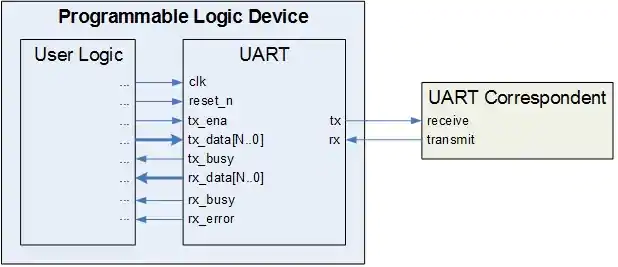
\includegraphics[scale=0.6]{img/theoretical-analysis/uart_core.png}
    \captionsetup{format=plain,justification=centering}
    \caption{Przykładowa struktura zewnętrzna bloku UART, źródło: \cite{uart_core}}
    \label{uart-core}
\end{figure}

W~pełni funkcjonalny układ UART można podzielić na trzy zasadnicze części: \textbf{generator sygnału taktującego}, moduł \textbf{nadawczy} oraz moduł \textbf{odbiorczy}. Pierwsza z~nich odpowiada za~wytworzenie dwóch sygnałów zegarowych - jednego o~częstotliwości równej częstotliwości transmisji (ang. \textit{baud ratate}) i~drugiego - taktowanego z~szybkością typowo ośmio- lub szesnastokrotnie większą (ang. \textit{oversampling rate}). Sygnał wolniejszy wykorzystywany jest przez moduł nadawczy do określania momentów transmisji kolejnych bitów. Z~kolei sygnał szybszy determinuje chwile próbkowania linii RX przez moduł odbiorczy. Skonstruowanie takiego generatora wymaga dwóch liczników oraz dwóch komparatorów. Potrzebne są również dwa rejestry przechowujące stosunki częstotliwości zegara systemowego do częstotliwości obu sygnałów generowanych. Rejestry te w~projekcie będą przechowywały wartości stałe, ponieważ zmienna szybkość transmisji nie jest wymagana.

Moduły nadawczy oraz odbiorczy stanowią dwóstanowe, synchroniczne automaty. Mogą się one znajdować w~stanie aktywnym (nadawanie/odbieranie) lub w~stanie bezczynnym (ang. \textit{idle}). Do nadawania wykorzystywany jest prosty rejestr przesówny, którego wyjście podłączone jest do linii TX natomiast wejście zegarowe (jak napisano wyżej) taktowane jest sygnałem \textit{baud}. Zamknięcie danych w~rejestrze oraz obliczenie bitu kontrolnego następuje po podaniu odpowiedniego stanu na dedykowanej linii wejściowej układu (TX\_EN). Analogiczna sytuacja zachodzi w~przypadku odbioru danych, przy czym sygnałem skutkującym przejściem moduł odbiorczego w~stan aktywny jest pojawienie się bitu startu na linii RX. Jest ona próbkowana z~częstotliwością równą częstotliwości sygnału \textit{oversampling}. Stan odbieranego bitu określany jest w~momencie połowy jego trwania na linii odbiorczej. Po zarejestrowaniu odpowiedniej liczby bitów sprawdzana jest parzystość danych oraz poprawność bitów stopu, po czym zakończenie danych sygnalizowe jest poprzez odpowiednią linię wyjściową układu (wraz z~ewentualnym ustawieniem linii błędu). Przykładowa struktura interfejsu urządzenia UART (wykorzystana w~tym projekcie) została przedstawiona na Rys. \ref{uart-core}
